% \fs and \fmax must be defined before calling this picture.
\def\fs{6.28}
\def\fmax{3.14}
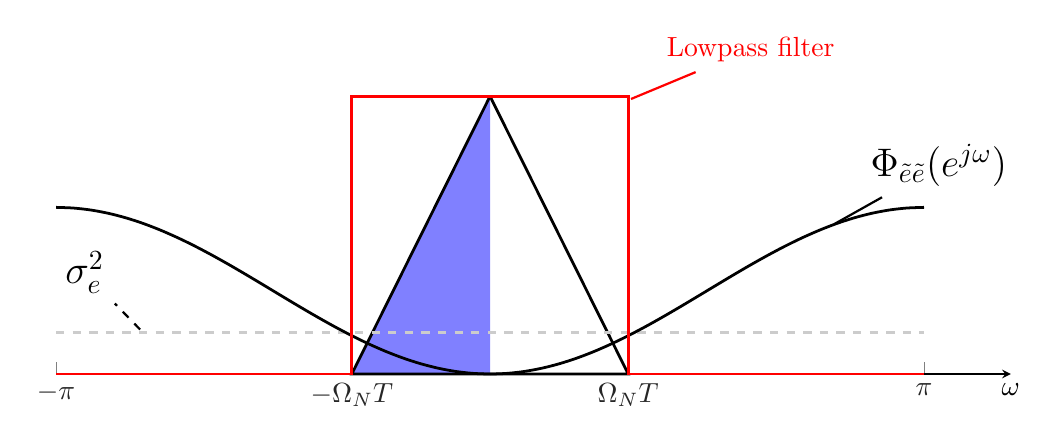
\begin{tikzpicture}
\begin{axis}[
	name=plot1,
	axis lines*=middle,
	enlargelimits = upper,
	clip=false,
	scale only axis,
	width=\textwidth,
	height=0.4\textwidth,
	ymin=0,	ymax=2.5, 
	hide y axis,
	xmin=-\fmax, xmax=\fmax,
	axis line style={->,>=stealth},
	xlabel={ $\omega$},
	%ylabel={ $X_c(j\Omega)$},
	every axis x label/.style={
		at={(ticklabel* cs:1)},
		anchor=north,
	},
	every axis y label/.style={
		at={(ticklabel* cs:0.8)},
		anchor=south,
		xshift=0.6cm,
	},
	ytick=2,
	xtick=\empty,
	yticklabel={ 1},
	xtick={-3.14, -1, 1, 3.14},
	xticklabels={ $-\pi$,  $-\Omega_NT$,  $\Omega_NT$,   $\pi$},
	every outer y axis line/.append style={white!15!black},
	every x tick label/.append style={font=\color{white!15!black}},
	legend style={draw=white!15!black,fill=white,legend cell align=left}]
	\addplot[solid, line width=1pt] coordinates {(0, 2) (1, 0) (0, 0)};
	\addplot[solid, line width=1pt, fill=blue!50] coordinates {(0, 2) (-1, 0) (0, 0)};
	
	\addplot[dashed, line width=1pt, black!20, domain=-\fmax:\fmax, samples=2] {0.3} node[pos=0.1, black, pin={[pin edge={black, thick}]135:{\Large \color{black} $\sigma_e^2$}}, inner sep=0pt] {};
	\addplot[smooth, line width=1pt, domain=-\fmax:\fmax, samples=51] {0.3*(2*sin(deg(x/2)))^2}
	node[pos=0.9, black, pin={[pin edge={black, thick}]45:{\Large $\Phi_{\tilde{e}\tilde{e}}(e^{j\omega})$}}, inner sep=0pt] {};
	
	\only<2-|handout:1>{
		\addplot[solid, red, line width=1pt] coordinates {(-3.14, 0) (-1, 0) (-1, 2) (1, 2) (1, 0) (3.14, 0)} node[pos=0.6, red, pin={[pin edge={red, thick}]45:{Lowpass filter}}, inner sep=0pt] {};
	}
\end{axis}
\end{tikzpicture}
